\subsubsection{Actors}
The actors of this system is the administator, a bartender or a barowner in charge of the music and the customer wanting to request and affect the music.

\textbf{Administrator}
Purpose:
A person in charge of the music, wants to be able to have control over the system, what kind of music is being enqueued and what is currently playing.


Characteristics:
Has a preference or a theme of music that the individual is following, set by the organisation or the invidual itself.

Possible usage:
adds restrictions, removes restriction, play music, stop music, play next track.

Diagram of possible usage, see \cref{fig:UsageAdmin}
\begin{figure}
  \centering
  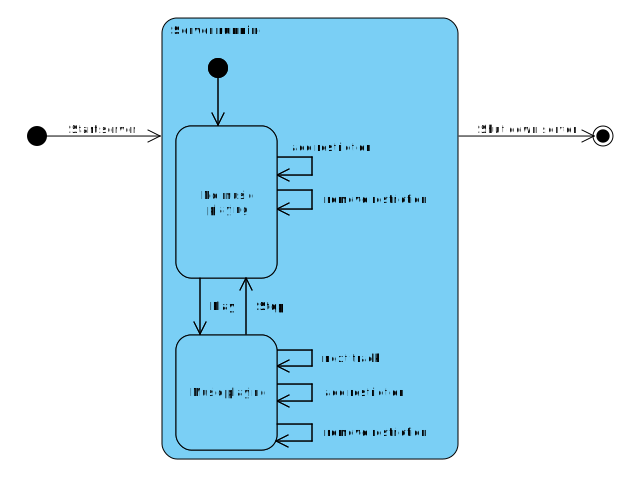
\includegraphics[width=0.7\linewidth]{Images/UsageAdmin.pdf}
  \caption{Usage for a administrator}
  \label{fig:UsageAdmin}
\end{figure}

\textbf{Customer}
Purpose:
Wants to listen to a prefered track at the venue, the individual is visiting.


Characteristics:
Music preferences may differ from the administrator set of preferences, or allowed themes of music, at a specific venue.

Possible usage:
Check in at venue, check out, vote for track, cancel vote.

Diagram of possible usage, see \cref{fig:UsageUser}
\begin{figure}
  \centering
  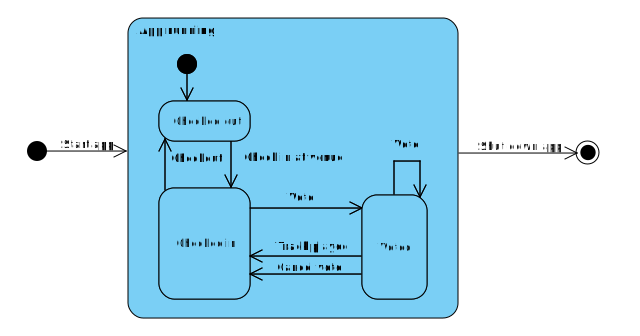
\includegraphics[width=0.7\linewidth]{Images/UsageUser.pdf}
  \caption{Usage for a customer}
  \label{fig:UsageUser}
\end{figure}